\documentclass[reqno]{amsart}
\usepackage{amsmath,amssymb,amsthm,amsfonts}
\usepackage{physics}
\usepackage{graphicx}
\usepackage{hyperref}
\usepackage{babel}
\usepackage{datetime}
\usepackage{ragged2e}
\usepackage{siunitx}
\usepackage{tikz}
\usetikzlibrary{quotes,angles}
\usepackage{quantikz}
\let\oldtocsection=\tocsection

\let\oldtocsubsection=\tocsubsection

\let\oldtocsubsubsection=\tocsubsubsection

\renewcommand{\tocsection}[2]{\hspace{0em}\oldtocsection{#1}{#2}}
\renewcommand{\tocsubsection}[2]{\hspace{1em}\oldtocsubsection{#1}{#2}}
\renewcommand{\tocsubsubsection}[2]{\hspace{2em}\oldtocsubsubsection{#1}{#2}}
\makeatletter
\renewcommand\subsection{\@startsection{subsection}{2}%
  \z@{.5\linespacing\@plus.7\linespacing}{-.5em}%
  {\normalfont\scshape}}
\makeatother


\DeclareMathOperator{\lcm}{lcm}
\newdateformat{monthyeardate}{%
  \monthname[\THEMONTH] \THEYEAR}
\numberwithin{equation}{section}
\numberwithin{figure}{section}
\tolerance=1
\emergencystretch=\maxdimen
\hyphenpenalty=10000
\hbadness=10000
\setcounter{tocdepth}{3}

\title{Quantum Computing}
\author[Elliott Ashby]{Elliott Ashby \\ Physics and Astronomy \\ University of Southampton}
\date{\monthyeardate\today}
% ----------------------------------------------------------------

\begin{document}
\begin{abstract}
    This report provides a high level overview of quantum computing. The history and development during the 20th century are discussed as well as the fundamental principals underpinning quantum computing such as qubits, superposition and entanglement. The report also discusses implementations of quantum computing such as quantum circuits and algorithms as well as the reasoning behind why those algorithms are needed to continue the current pace in the speed up of computation and even simulate physics impossible on a classical computer. Finally, the report discusses the criteria and requirements to build a quantum computer.
\end{abstract}
\maketitle
\tableofcontents
\section{Introduction}
\begin{justify}
Animals gain advantages in many ways, one of which is the exploitation of properties of the physical world. This has come to culmination in humans; in 1941 we saw the creation of the first programmable computer, the Z3, by Konrad Zuse, and in the following decades we have continually perfected this technology. The modern computer that we use today is, at its fundamental principals, identical to the Z3, performing binary operations on "bits" (a 1 or a 0) of data in order to encode useful computational results. \\

The Z3 used electromagnetic relays (600 in the arithmetic unit, 1,400 to store 64 words) and was close in size to the Stibitz BTL Model 1 or a large, floor-to-ceiling bookshelf. \cite{KonradZuseObituary} In the decades following the Z3, the space required to store and operate computer memory has decreased significantly, and as stated by Moore in 1965, "The complexity for minimum component costs has increased at a rate of roughly a factor of two per year." \cite{Moore1965} This has largely held true, thanks to increasingly smaller and smaller manufacturing processes. \\

As of 2022 the smallest transistors are of the order of 3nm, \cite{Samsung_2022} but when we shrink further down to 2nm or beyond, we begin to approach the size of the atom; at this scale, quantum effects are more pronounced and transistors can leak current due to gate direct tunnelling. \cite{2nmGateOxide} These effects limit the effectiveness of classical computers at this scale, and so we must look to new technologies to push the boundaries of computation.
\end{justify}
\section{An Overview of Key Concepts}
\subsection{A Brief History of Quantum Computing}
\begin{justify}
During the majority of the 20th century up until the early 1980s the fields of quantum mechanics and computer science were, for the most part, separate areas of study despite some crossover such as the laser. But in 1980, Paul Benioff proposed a quantum mechanical model of the computer and computation process \cite{Benioff1980} and additionally, in the same year, Yuri Manin proposed a similar model. \cite{Manin1980} In the following years, Richard Feynman wrote a paper suggesting that the use of quantum phenomena to perform computations could be more efficient for computer physics simulations than classical computers. \cite{Feynman1982} \\
2 years later, in 1984, Charles Bennett and Gilles Brassard continued to merge quantum mechanics and computer science by introducing quantum cryptography \cite{BennettBrassard1984} showing that a quantum key distribution can be used to secure communications. \\

Following the proposal of the quantum model of computation, quantum algorithms began to be developed, including Deutsch's algorithm in 1985, \cite{Deutsch1985} the Bernstein-Vazirani algorithm in 1993, \cite{BernsteinVazirani1993} and Simon's algorithm in 1994. \cite{Simon1994} Building on these papers, Peter Shor published his work on prime factorization quantum algorithms which had real world application breaking the RSA and Diffie-Hellman encryption algorithms. \cite{Shor1994} Just 2 years later in 1996, Lov Grover published his algorithm for database search \cite{Grover1996} and in the same year Seth Lloyd finally proved Feynman's conjecture that he proposed in 1982 that quantum computers (QCs) can be programmed to simulate any local quantum system. \cite{Lloyd1996} \\

The first QC to be built was in 1998; Isaac Chuang and Neil Gershenfeld along with Mark Kubinec implemented Grover's search algorithm with a 2-quantum bit (qubit) nuclear magnetic resonance (NMR) QC. \cite{ChuangGershefeldKubinec1998} In the years following, NMR QCs would increase in the number of qubits allowing for a 7-qubit QC to run Shor's algorithm in 2001. \cite{Vandersypen2001} \\

Since then, quantum computing has continued to grow, with new technologies and greater numbers of qubits. The most promising of these is the superconducting circuit used as a qubit. Originally proposed in 1999 by Yasunobu Nakamura, Yuri Pashkin and Jaw-Shen Tsai, \cite{NakamuraPashkinTsai1999} and shown to be viable for greater application in 2007 by Jelle Plantenberg, P.C. de Groot, C.J.P.M. Harmans and Hans Mooij by demonstrating the controlled-NOT gate, \cite{PlantenbergGrootHarmansMooij2007} superconducting qubits have become the focus of many large companies such as IBM and Google. \\

As of 2024, the QC with the most number of qubits is actually not a superconducting QC, but an atomic array QC built by Atom Computing in 2023 \cite{Atom2023, Atom2024} with a reported 1,180 qubits. However, since atomic array QCs are much newer than superconducting QCs, they have less general support for quantum algorithms; the largest superconducting QC as of 2024 is IBM's Condor with 1121 qubits. \cite{IBM2023, AbuGhanem2024} \\

The field of quantum computing is still in its infancy, but with promising results and continued growth, it is likely that QCs will become more relevant in the coming years.
\end{justify}

\subsection{Limitations of Classical Computers and the Need for Quantum Computing}
\subsubsection{Public-key Cryptography and Factorization of Big Numbers} \label{sec:PublickeyCryptography}
\begin{justify}
In 1976, Whitfield Diffie and Martin Hellman published their paper on new directions in cryptography, \cite{DiffieHellman1976} introducing to the general public the concept of public-key cryptography; a method of encryption that uses a pair of keys, public and private, to encrypt and decrypt messages. With the public key, one can encrypt a message that only the private key can decrypt. 2 years later in 1978, Ron Rivest, Adi Shamir and Leonard Adleman published their paper on the "RSA" algorithm, named after their initials, that provides a method for generation of the keys. \cite{RSA1978}\\

The problem of breaking the RSA algorithm is one of finding the prime factors of a large integer. This is difficult to solve for classical computers; the best known algorithm, the general number field sieve (GNFS) \cite{Briggs1998} runs in sub-exponential time, with a time complexity of:
    \begin{equation*}
        O\left(\exp\left[\left(\frac{64}{9}\right)^{1/3}(\log n)^{1/3}(\log \log n)^{2/3}\right]\right) 
    \end{equation*}
    where $n$ is the number to be factorized. If we were to use an $n$ of $2^{2048}$, we would yield a number of operations roughly $\num{1.53e35}$. On a 5GHz CPU on a single thread, this would take $\num{9.72e17}$ years, a long enough time that the RSA algorithm would be considered secure. \\

    However in 1994, Peter Shor published his quantum algorithm for prime factorization \cite{Shor1994} now known as Shor's Algorithm. Shor suggests that a QC could be able to factorize a number in polynomial time $O(\log n)$. The fastest current implementation is of $O((\log n)^{2}(\log \log n))$ \cite{Beckman1996, HarveyHoeeven2021} yielding a number of operations $\num{1.46e7}$. This is a significant speed up over the GNFS and implies that the RSA algorithm is no longer secure. Among security experts, security through obscurity is not considered a valid form of security, \cite{ScarfoneJansenTracy2008} and as such, the need for further research into quantum computing and quantum-resistant cryptography is clear. Shor's Algorithm is discussed further in section \ref{sec:ShorsAlgorithm}.
\end{justify}
\subsubsection{Brute-force Search}
\begin{justify}
Brute-force search is a method of problem solving that involves systematically generating and testing all possible solutions to a problem. That is to say, brute-force search find the single item that satisfies some condition in a unsorted database of $n$ items. Once a single item has been examined, its ability to satisfy the condition can be determined in one step and as such, the most efficient classical algorithms may only determine the correct item in $O(n)$ time, averaging $n/2$ operations. \\

In 1996, Lov Grover published his quantum algorithm for database search \cite{Grover1996} now known as Grover's Algorithm. Grover's Algorithm is able to find this single item in only $O(\sqrt{n})$ steps, and although not a polynomial time speed up, it is still a significant speed up over classical algorithms. Grover's Algorithm is possible since, quantum mechanical systems can be in a superposition of states and simultaneously evaluate the conditions for multiple items in the database. \\

A year later in 1997, Grover's Algorithm was shown to be asymptotically optimal by Charles Bennett, Ethan Bernstein, Gilles Brassard and Umesh Vazirani. \cite{BennettBernsteinBrassardVazirani1997} An algorithm is said to be asymptotically optimal if it, for large inputs, performs at worst a constant factor worse than the best possible algorithm.
\end{justify}
\subsubsection{Simulation of Quantum Systems}
\begin{justify}
Can physics be simulated on a classical computer? In 1982, Richard Feynman states that it is certainly not possible to simulate quantum systems on a classical computer without infinite time. \cite{Feynman1982} \\

If we wish to simulate a single particle, $\psi$ as a function of $x$ and $t$, its probability density can be determined classically using numerical methods. \cite{Schroedinger1926} However, if we wish to simulate $n$ particles, the new state of the system is given by some function $\Psi(x_{1}, x_{2}, \ldots, x_{n}, t)$. Describing all of these states would require a $k$-digit number for every configuration of the system, for every arrangement of the $n$ values of $x$. Then, if there are $N$ points in space and each point in space has its own information such as electric fields, $n$ is of order $N$, so there would be $N^N$ configurations. Since there are too many variables, it cannot be simulated with a classical computer; there are more variables than estimated atoms in the universe! Computing this classically would require to discretize $x$ and $t$ to make any results exact. To do this requires the discarding of terms that are too small, for example if we choose to only take $k$ digits of precision, we must discard probabilities that are less than $2^{-k}$. This is not a problem for a small number of particles, but as the number of particles increases to $n$, the more terms we discard, no matter their validity. \\

Feynman presents that discretizing presents some problems, for example taking the electric field at some point below a certain amount, would in turn suggest that it is not there at all. This is not the case, we know it to be quantized. By discretizing, we are not simulating the correct equations that reflect reality. \\

This leaves only one option, to simulate quantum systems on a QC. Feynman's conjecture was backed up by Seth Lloyd later in 1996 \cite{Lloyd1996} stating that a mere 30 or 40 qubits would be enough to simulate a quantum simulations of multidimensional fermionic systems like the Hubbard model \cite{Hubbard1963} that prove resistant to conventional computers. \\
\end{justify}
\subsection{Quantum Bits and Superposition} \label{sec:QubitsandSuperposition}
\begin{justify}
    The bit is the smallest building block of information of classical information. Similarly, the qunatum bit or qubit is the equivalent for quantum information theory. \cite{Aaronson2013} While the qubit can be represented by physical systems such as photons, electrons or atoms, for now we will consider the qubit as a abstract concept. \\

    While a classical bit has a state of either 0 or 1, qubits similarly have a state of $\ket{0}$ or $\ket{1}$ which correspond to the classical states respectively. There is one key difference however, instead of being exclusively in one state or the other, a qubit can also be in a \textit{linear combination} of states also known as a \textit{superposition}. That is to say, a qubit can be represented as:
    \begin{equation}
        \ket{\psi} = \alpha\ket{0} + \beta\ket{1} \label{eq:qubit}
    \end{equation}
where $\alpha$ and $\beta$ are complex numbers and $|\alpha|^{2} + |\beta|^{2} = 1$. These states however, are not observable, to retrieve information from a qubit, it must be measured. Doing so we get either 0 or 1 with a probability of $|\alpha|^{2}$ and $|\beta|^{2}$ respectively. An example of this could be for a qubit to be in the following states:
    \begin{eqnarray}
        \ket{+} &=& \frac{\ket{0} + \ket{1}}{\sqrt{2}} \label{eqn:+} \\
        \ket{-} &=& \frac{\ket{0} - \ket{1}}{\sqrt{2}} \label{eqn:-}
    \end{eqnarray}
which we have denoted as $\ket{+}$ and $\ket{-}$.

If we wish to, we can also represent a single qubit using a \textit{Bloch sphere} \cite{FeynmanRichardVernon1957}; a sphere with radius 1 and the poles representing the 2 states $\ket{0}$ and $\ket{1}$. We can rewrite Equation (\ref{eq:qubit}) as:
    \begin{equation}
        \ket{\psi} = \cos\left(\frac{\theta}{2}\right)\ket{0} + e^{i\varphi}\sin\left(\frac{\theta}{2}\right)\ket{1}
    \end{equation}
where $\theta$ and $\phi$ are the angles of the Bloch sphere shown in Figure \ref{fig:BlochSphere}. Operations on single qubits can be represented as rotations on the Bloch sphere, which is a useful way to visualize quantum operations. \\
    \begin{figure}[h]
        \centering
        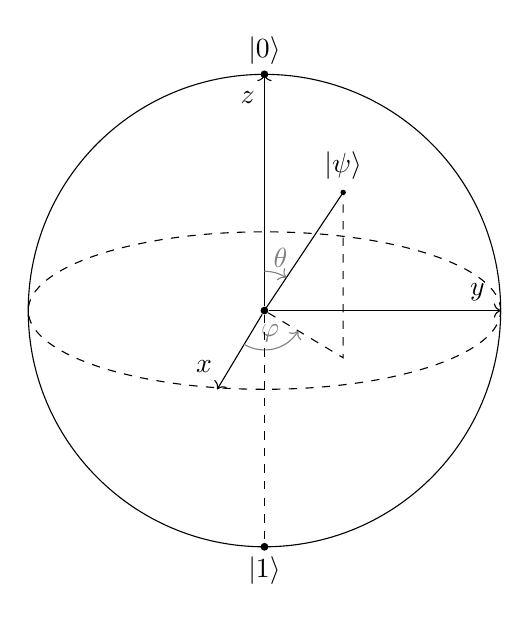
\begin{tikzpicture}

              % Define radius
              \def\r{3}

              % Bloch vector
              \draw (0, 0) node[circle, fill, inner sep=1] (orig) {} -- (\r/3, \r/2) node[circle, fill, inner sep=0.7, label=above:$\ket{\psi}$] (phi) {};
              \draw[dashed] (orig) -- (\r/3, -\r/5) node (phinode) {} -- (phi);

              % Sphere
              \draw (orig) circle (\r);
              \draw[dashed] (orig) ellipse (\r{} and \r/3);

              % Axes
              \draw[->] (orig) -- ++(-\r/5, -\r/3) node[pos=0.9, above left] (x1) {$x$};
              \draw[->] (orig) -- ++(\r, 0) node[pos=0.9, above] (x2) {$y$};
              \draw[->] (orig) -- ++(0, \r) node[pos=0.9, left] (x3) {$z$};

              % Angles
              % \pic["$\phi$", draw=gray, text=gray, ->] {angle = x1--orig--phi};
              % \pic["$\theta$", draw=gray, text=gray, <-, angle eccentricity=1.4] {angle = a--orig--x3};
          	  \path (orig) ++(-\r/10, -\r/6) coordinate (phi_start); % Start point for phi
              \pic [draw=gray, text=gray, ->, "$\varphi$"] {angle = phi_start--orig--phinode};
              \path (orig) ++(0, \r/2) coordinate (theta_start); % Start point for theta
              \pic [draw=gray, text=gray, <-, "$\theta$", angle eccentricity=1.4] {angle = phi--orig--theta_start};

              % Kets at poles with nodes
              \node[circle, fill, inner sep=1] at (0, \r) {}; % North pole node
              \node[above] at (0, \r) {$|0\rangle$};          % Label for north pole
              \node[circle, fill, inner sep=1] at (0, -\r) {}; % South pole node
              \node[below] at (0, -\r) {$|1\rangle$};
              \draw[dashed] (orig) -- (0, -\r); % Dashed line orig and south pole

        \end{tikzpicture}
        \caption{The Bloch Sphere}
        \label{fig:BlochSphere}
    \end{figure}

    Despite the fact that a single qubit has an infinite number of possible states (all possible values of $\alpha$ and $\beta$), we cannot use a qubit to store an infinite amount of data. This is because in order to extract any information from a qubit it must be measured; measurement results in a collapse from its superposition of $\ket{0}$ and $\ket{1}$ to either 0 or 1. This means that any further measurements are guaranteed to yield the same result. For example, if measurement of $\ket{-}$ gives 1, then any additional measurements must also give 1. \\
\end{justify}
\subsection{Quantum Superposition of Multiple Qubits and Entanglement}
\begin{justify}
    Just as a single qubit can be in a superposition of states, multiple qubits can be in a superposition of states. For example, a 2-qubit system can be in a superposition of 4 states:
    \begin{equation}
        \ket{\psi} = \alpha_{00}\ket{00} + \alpha_{01}\ket{01} + \alpha_{10}\ket{10} + \alpha_{11}\ket{11} \label{eq:entanglement}
    \end{equation}
    where $\alpha_{00}$, $\alpha_{01}$, $\alpha_{10}$ and $\alpha_{11}$ are complex numbers and $|\alpha_{00}|^{2} + |\alpha_{01}|^{2} + |\alpha_{10}|^{2} + |\alpha_{11}|^{2} = 1$. Similarly to a single qubit, the probability of measuring a state $\ket{xy}$ is $|\alpha_{xy}|^{2}$. However we could potentially only measure one of the two qubits, collapsing that one but not the other. If we measured the first qubit to be 1, the new state of the system would then be:
    \begin{equation}
        \ket{\psi'} = \frac{\alpha_{10}\ket{10}+\alpha_{11}\ket{11}}{\sqrt{\abs{\alpha_{10}}^{2} + \abs{\alpha_{11}}^{2}}}
    \end{equation}
    But this raises a strange point, as pointed out by Albert Einstein, Boris Podolsky and Nathan Rosen in 1935 \cite{EinsteinPodolskyRosen1935} that the measurement of one qubit can determine the state of another qubit simultaneously. Einstein Podolsky and Rosen suggested that this was a problem with quantum mechanics, saying that, "No reasonable definition of reality could be expected to permit this." This is known as the \textit{EPR-paradox}. However, later in 1964 John Bell suggested that, using a refinement on the EPR-paradox by David Bohm and Yakir Aharonov \cite{BohmAharonov1957} showing that the EPR-paradox could be tested experimentally, that there "must be a mechanism whereby the setting of one measuring device can influence the reading of another instrument, however remote." \cite{Bell1964} This is known as \textit{quantum entanglement}. From these results we can derive states of equal coefficients and a single measurement from Equation (\ref{eq:entanglement}). These are known as the \textit{Bell states} or \textit{EPR pairs}: 
        \begin{eqnarray}
            \ket{\Phi^{+}} &=& \frac{\ket{00} + \ket{11}}{\sqrt{2}} \label{eqn:bellphi+} \\
            \ket{\Phi^{-}} &=& \frac{\ket{00} - \ket{11}}{\sqrt{2}} \label{eqn:bellphi-} \\
            \ket{\Psi^{+}} &=& \frac{\ket{01} + \ket{10}}{\sqrt{2}} \label{eqn:bellpsi+} \\
            \ket{\Psi^{-}} &=& \frac{\ket{01} - \ket{10}}{\sqrt{2}} \label{eqn:bellpsi-} 
        \end{eqnarray}
They form the \textit{Bell basis} of the four-dimensional Hilbert space for 2 qubits.
\end{justify}
\section{Quantum Circuits}
\subsection{Quantum Gates}
\begin{justify}
    Classical computers are made of wires and logic gates. Wires move bits around while logic gates manipulate input bits and produce output bits. In order to build a QC, there must be a similar model of computation allowing for input qubits to be converted to output qubits but with one key difference; the QC must be reversible. This is because the laws of quantum mechanics are reversible in time, and as such, any quantum operation must be reversible. These observations were first made by Charles Bennett in 1973 \cite{Bennett1973} and developed further by Edward Fredkin and Tommaso Toffoli as well as Bennett separately in 1982. \cite{FredkinToffoli1982, Bennett1982} Feynman continues this work, discussing possible Hamiltonions for QCs in 1986. \cite{Feynman1986} \\

To define a gate classically, we can use a truth table. For example, the truth tables for the NOT and AND gates are:
    \begin{eqnarray}
        \begin{array}{c|c}
            \text{NOT} & \text{AND}\\
            \hline
            \begin{array}{c|c}
                \text{a} & \text{a'} \\
                \hline
                0 & 1 \\
                1 & 0
            \end{array} &
            \begin{array}{cc|c}
                \text{a} & \text{b} & \text{a'} \\
                \hline
                0 & 0 & 0 \\
                0 & 1 & 0 \\
                1 & 0 & 0 \\
                1 & 1 & 1
            \end{array}
        \end{array}
    \end{eqnarray}
    If at a minimum we wish QCs to be able to perform the same operations as classical computers, they must be able to perform these 2 operations since they are the minimum required for a Turing complete classical computer (either OR or AND are required). \cite{CopiCohenMcMahon2011} In order to convert these into quantum gates we must make sure that they are reversible, that is to say, for a quantum mechanical system they must be unitary operators. (An operator $U$ is unitary if $U^{\dagger}U = UU^{\dagger} = I$ and $U^{\dagger} = U^{-1}$ where $I$ is the identity matrix.) \\

For NOT, we can define the operation as:
    \begin{equation}
        \alpha\ket{0} + \beta\ket{1} \rightarrow \alpha\ket{1} + \beta\ket{0}
    \end{equation}
where we can write the state as a column vector of complex coefficients:
    \begin{equation}
        \begin{bmatrix}
            \alpha \\
            \beta
        \end{bmatrix}
        \label{eq:qubitmatrix}
    \end{equation}
where the top entry is the complex coefficient of $\ket{0}$ and the bottom entry is the complex coefficient of $\ket{1}$. The NOT gate can then be represented as:
    \begin{equation}
        X \equiv \begin{bmatrix}
                    0 & 1 \\
                    1 & 0
                \end{bmatrix}
                \label{eq:NOTmatrix}
    \end{equation}
If we apply the NOT gate to the state (\ref{eq:qubitmatrix}), we get:
    \begin{equation}
        X\begin{bmatrix}
            \alpha \\
            \beta
        \end{bmatrix} = \begin{bmatrix}
                            0 & 1 \\
                            1 & 0
                        \end{bmatrix}\begin{bmatrix}
                                        \alpha \\
                                        \beta
                                    \end{bmatrix} = \begin{bmatrix}
                                                        \beta \\
                                                        \alpha
                                                    \end{bmatrix}
    \end{equation}
which is also easily shown to be unitary. \\

AND however is more tricky. Looking at its truth table, we can see that it is not reversible. An output of $0$ could be the result of three different inputs. However, in 1981 Toffoli published a paper discussing the construction of reversible primitives to create an arbitrary invertible combinatorial function. \cite{Toffoli1981} The three primitives required are: NOT, CONTROLLED NOT (CNOT) and CONTROLLED CONTROLLED NOT (CCNOT). The truth tables for CNOT and CCNOT are:
    \begin{eqnarray}
        \begin{array}{c|c}
            \text{CNOT} & \text{CCNOT} \\
            \hline
            \begin{array}{cc|cc}
                \text{a} & \text{b} & \text{a'} & \text{b'} \\
                \hline
                0 & 0 & 0 & 0 \\
                0 & 1 & 0 & 1 \\
                1 & 0 & 1 & 1 \\
                1 & 1 & 1 & 0
            \end{array} &
            \begin{array}{ccc|ccc}
                \text{a} & \text{b} & \text{c} & \text{a'} & \text{b'} & \text{c'} \\
                \hline
                0 & 0 & 0 & 0 & 0 & 0 \\
                0 & 0 & 1 & 0 & 0 & 1 \\
                0 & 1 & 0 & 0 & 1 & 0 \\
                0 & 1 & 1 & 0 & 1 & 1 \\
                1 & 0 & 0 & 1 & 0 & 0 \\
                1 & 0 & 1 & 1 & 0 & 1 \\
                1 & 1 & 0 & 1 & 1 & 1 \\
                1 & 1 & 1 & 1 & 1 & 0 \\
            \end{array}
        \end{array}
    \end{eqnarray}
Already we can see that using CCNOT, by setting $c = 0$, $c' = 1$ only if $a = b = 1$. This is the AND gate. However, crucially the CCNOT gate is reversible due to the fact that it has a unique output for each input. \\

For CNOT we can define the operation as:
    \begin{equation}
        \alpha\ket{00} + \beta\ket{01} + \gamma\ket{10} + \delta\ket{11} \rightarrow \alpha\ket{00} + \beta\ket{01} + \delta\ket{10} + \gamma\ket{11}
    \end{equation}
The CNOT gate can then be represented as:
    \begin{equation}
        CNOT \equiv \begin{bmatrix}
                    1 & 0 & 0 & 0 \\
                    0 & 1 & 0 & 0 \\
                    0 & 0 & 0 & 1 \\
                    0 & 0 & 1 & 0
                \end{bmatrix}
    \end{equation}

CCNOT is similar to CNOT, but with an additional control qubit. We can define the operation as:
    \begin{equation}
        \begin{split}
            &\alpha\ket{000} + \beta\ket{001} + \gamma\ket{010} + \delta\ket{011} + \epsilon\ket{100} + \zeta\ket{101} + \eta\ket{110} + \theta\ket{111} \\ \rightarrow
            &\alpha\ket{000} + \beta\ket{001} + \gamma\ket{010} + \delta\ket{011} + \epsilon\ket{100} + \zeta\ket{101} + \eta\ket{111} + \theta\ket{110}
        \end{split}
    \end{equation}
The CCNOT gate can then be represented as:
    \begin{equation}
        CCNOT \equiv \begin{bmatrix}
                    1 & 0 & 0 & 0 & 0 & 0 & 0 & 0 \\
                    0 & 1 & 0 & 0 & 0 & 0 & 0 & 0 \\
                    0 & 0 & 1 & 0 & 0 & 0 & 0 & 0 \\
                    0 & 0 & 0 & 1 & 0 & 0 & 0 & 0 \\
                    0 & 0 & 0 & 0 & 1 & 0 & 0 & 0 \\
                    0 & 0 & 0 & 0 & 0 & 1 & 0 & 0 \\
                    0 & 0 & 0 & 0 & 0 & 0 & 0 & 1 \\
                    0 & 0 & 0 & 0 & 0 & 0 & 1 & 0
                \end{bmatrix}
    \end{equation}

    While viewing the gates in their matrix forms is useful for tracking the operations each gate makes, a more intuitive way could be to present the gates as circuits more akin to classical computing. This can be seen in Figures \ref{fig:NOT}, \ref{fig:CNOT} and \ref{fig:CCNOT}. \\
    \begin{figure}[h]
        \centering
        \begin{quantikz}
            \lstick{$\ket{a}$} & \gate{X} & \rstick{$\ket{a'}$} \qw
        \end{quantikz}
        \caption{Circuit for NOT}
        \label{fig:NOT}
    \end{figure}
    \begin{figure}[h]
        \centering
        \begin{quantikz}
            \lstick{$\ket{a}$} & \ctrl{1} & \rstick{$\ket{a}$} \qw \\
            \lstick{$\ket{b}$} & \targ{} & \rstick{$\ket{a, a \oplus b}$} \qw
        \end{quantikz}
        \caption{Circuit for CNOT}
        \label{fig:CNOT}
    \end{figure}
    \begin{figure}[h]
        \centering
        \begin{quantikz}
            \lstick{$\ket{a}$} & \ctrl{1} & \rstick{$\ket{a}$} \qw \\
            \lstick{$\ket{b}$} & \ctrl{1} & \rstick{$\ket{b}$} \qw \\
            \lstick{$\ket{c}$} & \targ{} & \rstick{$\ket{a, b, c \oplus (a \land b)}$} \qw
        \end{quantikz}
        \caption{Circuit for CCNOT}
        \label{fig:CCNOT}
    \end{figure}
\\

    With these gates, any classical circuit is constructable. For example, the full adder circuit can be constructed using CNOT and CCNOT gates as shown in Figure \ref{fig:FullAdder}.
    \begin{figure}[h]
        \centering
        \begin{quantikz}
            \lstick{$\ket{A}$} & \ctrl{1} & \ctrl{1} & \qw & \qw & \ctrl{1} & \rstick{$\ket{A}$} \qw \\
            \lstick{$\ket{B}$} & \ctrl{2} & \targ{} & \ctrl{1} & \ctrl{1} & \targ{} & \rstick{$\ket{B}$} \qw \\
            \lstick{$\ket{C_{in}}$} & \qw & \qw & \ctrl{1} & \targ{} & \qw & \rstick{$\ket{S}$} \qw \\
            \lstick{$\ket{0}$} & \targ{} & \qw & \targ{} & \qw & \qw & \rstick{$\ket{C_{out}}$} \qw
        \end{quantikz}
        \caption{Circuit for Full Adder where $S$ is the sum and $C_{in/out}$ is the carry in/out}
        \label{fig:FullAdder}
    \end{figure}
\\

However, quantum circuits are not limited to classical circuits; any unitary matrix, a theoretically infinite amount, \cite{Barenco1995} can be used as a quantum logic gate. The most obvious of which, for quantum mechanics would be the Identity and the Pauli matrices \cite{Pauli1925} which act on a single qubit state, one of which we have already defined in Equation (\ref{eq:NOTmatrix}).
    \begin{eqnarray}
        &I& = \begin{bmatrix}
                1 & 0 \\
                0 & 1
                \end{bmatrix} \\
        X = &\sigma_{x}& = \begin{bmatrix}
                            0 & 1 \\
                            1 & 0
                            \end{bmatrix} \\
        Y = &\sigma_{y}& = \begin{bmatrix}
                            0 & -i \\
                            i & 0
                            \end{bmatrix} \\
        Z = &\sigma_{z}& = \begin{bmatrix}
                            1 & 0 \\
                            0 & -1
                            \end{bmatrix}
    \end{eqnarray}
where X is the NOT gate and Y and Z can be visualized as rotations around the Bloch sphere. Y maps $\ket{0}$ to $i\ket{1}$ and $\ket{1}$ to $-i\ket{0}$, while Z maps $\ket{0}$ to $\ket{0}$ and $\ket{1}$ to $-\ket{1}$. Z can be especially useful as it flips the phase of the single qubit state. We could generalize the Z gate to the Phase shift gate:
    \begin{equation}
        P(\varphi) = \begin{bmatrix}
                    1 & 0 \\
                    0 & e^{i\varphi}
                    \end{bmatrix}
    \end{equation}
and redefine the Z gate as $P(\pi)$. However, $P(\varphi)$ is not Hermitian except for if $\varphi = n\pi, n \in \mathbb{Z}$. This means that it will not corresond to a difference in measurement and purely operates as change of relative phase. \\

We could also generalize the CNOT gate to a CU gate where U is any single qubit gate. This is done by applying the U gate to the target qubit if the control qubit is 1. The CU gate can be represented as:
    \begin{equation}
        CU = \begin{bmatrix}
                I & 0 \\
                0 & U
            \end{bmatrix} = \begin{bmatrix}
                                1 & 0 & 0 & 0 \\
                                0 & 1 & 0 & 0 \\
                                0 & 0 & u_{00} & u_{01} \\
                                0 & 0 & u_{10} & u_{11}
                            \end{bmatrix}
    \end{equation}
where $u_{ij}$ are the elements of the matrix $U$. \\

In Equations (\ref{eqn:+}, \ref{eqn:-}) 2 states were introduced $\ket{+}$ and $\ket{-}$, where the state has an equal chance of collapsing to either $\ket{0}$ or $\ket{1}$. If we wanted to create these states from an input state, say $\ket{0}$ or $\ket{1}$, we could use the following gate:
    \begin{equation}
        H = \frac{1}{\sqrt{2}}\begin{bmatrix}
                                1 & 1 \\
                                1 & -1
                            \end{bmatrix}
    \end{equation}
    which would map $\ket{0}$ to $\ket{+}$ and $\ket{1}$ to $\ket{-}$. This gate is known as the Hadamard gate after Jaques Hadamard. \cite{Hadamard1893} For example, if we apply the Hadamard gate to $\ket{0}$, we get:
    \begin{equation}
        H\ket{0} = \frac{1}{\sqrt{2}}\begin{bmatrix}
                                        1 & 1 \\
                                        1 & -1
                                    \end{bmatrix}\begin{bmatrix}
                                                    1 \\
                                                    0
                                                \end{bmatrix} = \frac{1}{\sqrt{2}}\begin{bmatrix}
                                                                                    1 \\
                                                                                    1
                                                                                \end{bmatrix} = \ket{+}
    \end{equation}
Creating a superposition of states is a key part of the power of quantum computing, as it allows for the simultaneous evaluation of multiple states. This will be discussed further in Section \ref{sec:QuantumAlgorithms}. \\

Finally, in order to use any information we have computed, we must measure our quantum states. This can be done by measuring (projecting) the state onto a basis. Since this operation is irreversable, it is not a unitary operation and as such, not a quantum gate; implementations of measurement will depend on the physical system used to implement the QC. Using the visual representation of quantum circuits we can represent measurement as shown in Figure \ref{fig:Measurement}.
    \begin{figure}[h]
        \centering
        \begin{quantikz}
           & \meter{} &\setwiretype{c}
        \end{quantikz}
        \caption{Symbol for measurement of a qubit. The incoming single wire represents that it carries a qubit while the outgoing double wire represents that it carries a classical bit.}
        \label{fig:Measurement}
    \end{figure}
\end{justify}
\subsection{Copying a Qubit}
\begin{justify}
    Using a classical CNOT gate, it is elementary to copy a single bit; we take in an unknown bit $x$ and a bit initialised to $0$, if $x$ is $0$ then the output is $0$ and if $x$ is $1$ then the output is $1$. Suppose we do the same with an unknown qubit $\ket{\psi}$ and a qubit $\ket{0}$:
    \begin{equation}
        \ket{\psi}\ket{0} = \alpha\ket{00} + \beta\ket{10} \xrightarrow{\text{CNOT}} \alpha\ket{00} + \beta\ket{11} \label{eqn:copy}
    \end{equation}
    Therefore we have changed the state of of $\ket{\psi}\ket{0}$ based on the value of $\ket{0}$; we have classically copied information. However, for the general case, where neither qubit is known and the operation must be reversible, a copied qubit would be in the state:
    \begin{equation}
        \ket{\psi}\ket{\psi} = \alpha^{2}\ket{00} + \alpha\beta\ket{01} + \alpha\beta\ket{10} + \beta^{2}\ket{11}
    \end{equation}
    where there is an output for every unique input. However, this is not the case for Equation (\ref{eqn:copy}) unless $\alpha\beta=0$; cloning a qubit is not possible. This is known as the \textit{no-cloning theorem} and was first proven by Wootters and Zurek in 1982. \cite{WoottersZurek1982}. \\

    Despite not being able to clone a qubit our output from Equation (\ref{eqn:copy}) is still useful. You may notice that it looks similar to out Bell states from Equations (\ref{eqn:bellphi+}, \ref{eqn:bellphi-}, \ref{eqn:bellpsi+}, \ref{eqn:bellpsi-}). In fact, we can make a circuit using Hadamard to create a Bell state from 2 qubits. This is shown in Figure \ref{fig:BellState}.
    \begin{figure}[h]
        \begin{eqnarray*}
            \begin{array}{c|c}
                \text{Input xy} & \text{Output z} \\ 
                \hline
                \ket{00} & \ket{\Phi^{+}} \\
                \ket{01} & \ket{\Phi^{-}} \\
                \ket{10} & \ket{\Psi^{+}} \\
                \ket{11} & \ket{\Psi^{-}}
            \end{array} \\
            \begin{quantikz}
                \lstick{x} & \gate{H} & \ctrl{1} & \rstick[2]{z} \qw \\
                \lstick{y} & \qw & \targ{} & \rstick{} \qw
            \end{quantikz}
        \end{eqnarray*}
        \caption{Circuit for creating a Bell state}
        \label{fig:BellState}
    \end{figure}
\end{justify}
\section{Quantum Algorithms and Parallelism} \label{sec:QuantumAlgorithms}
\subsection{Deutsch-Jozsa Algorithm}
\begin{justify}
    Originally proposed by David Deutsch and Richard Jozsa in 1992 and updated by Richard Cleve, Artur Ekert, Chiara Macchiavello and Michele Mosca in 1998, \cite{DeutschJozsa1992, CleveEkertMacchiavelloMosca1998} the Deutsch-Jozsa algorithm is one of the earliest examples of a quantum algorithm that outperforms its classical counterpart and while it doesnt have much practical use, it clearly shows the parallelism inherent in quantum computing. \\

    The problem that the algorithm aims to solve is as follows: We have a QC ($U_{f}$) of which we have no knowledge of its internal workings. It implements some function $f: \{0, 1\}^{n} \rightarrow \{0, 1\}$ which takes n-bit binarary values as inputs and outputs either a 0 or a 1. Lastly we assume that the function is either constant (always outputs 0 or 1 no matter the input) or balanced (outputs 0 and 1 for half the inputs each). We then wish to determine if the function is constant or balanced. \\

The classical solution to this problem would be to evaluate the function for all possible inputs and if we find that the function is not constant, then it must be balanced. This would require $2^{n-1} + 1$ evaluations of the function. However, the Deutsch-Jozsa algorithm can solve this problem with only 1 evaluation of the function. The algorithm can be seen in Figure \ref{fig:DeutschJozsa}. \\
    \begin{figure}[h]
        \centering
        \begin{quantikz}
            \lstick{$\ket{0}$} & \qwbundle{n} \slice{$\ket{\Psi_{0}}$} & \gate{H^{\otimes n}} \slice{$\ket{\Psi_{1}}$} & \gate[2][2cm]{U_{f}}\gateinput{$x$}\gateoutput{$x$} \slice{$\ket{\Psi_{2}}$} & \gate{H^{\otimes n}} \slice{$\ket{\Psi_{3}}$} & \meter{} \\
            \lstick{$\ket{1}$} & \qw & \gate{H} & \gateinput{$y$}\gateoutput{$y\oplus f(x)$} & \qw & \qw
        \end{quantikz}
        \caption{Circuit for the Deutsch-Jozsa algorithm}
        \label{fig:DeutschJozsa}
    \end{figure}

Walking though the algorithm step by step:
    \begin{enumerate}
        \item Our initial state $\ket{\Psi_{0}}$ is with $n+1$ qubits, $n$ of which are in the state $\ket{0}$ and the last in the state $\ket{1}$. This can also be written as $\ket{0}^{\otimes n}\ket{1}$.
            \begin{equation}
                \ket{\Psi_{0}} = \ket{0}^{\otimes n}\ket{1}
            \end{equation}
        \item We then apply the Hadamard gate to all qubits:
            \begin{equation}
                H\ket{\Psi_{0}} = \ket{\Psi_{1}} = \sum\limits_{x=0}^{2^{n}-1}\frac{\ket{x}}{\sqrt{2^{n}}}\left[\frac{\ket{0} - \ket{1}}{\sqrt{2}}\right]
            \end{equation}
        \item We then apply the oracle $U_{f}$ which acts like $\ket{x} \rightarrow (-1)^{f(x)}\ket{x}$:
            \begin{equation}
                U_{f}\ket{\Psi_{1}} = \ket{\Psi_{2}} = \sum\limits_{x}\frac{(-1)^{f(x)}\ket{x}}{\sqrt{2^{n}}}\left[\frac{\ket{0} - \ket{1}}{\sqrt{2}}\right]
            \end{equation}
        \item We then apply the Hadamard gate to the first $n$ qubits:
            \begin{equation}
                \ket{\Psi_{3}} = \sum\limits_{z}\sum\limits_{x}\frac{(-1)^{x \cdot z + f(x)}\ket{z}}{\sqrt{2^{n}}}\left[\frac{\ket{0} - \ket{1}}{\sqrt{2}}\right] \label{eq:finalstate}
            \end{equation}
            since for a single qubit $H\ket{x} = \frac{1}{\sqrt{2}}\sum_{z}(-1)^{x \cdot z}\ket{z}$.
        \item Finally, we measure $\ket{\Psi_{3}}$. In order for the function $f$ to be constant, the state must either be $\ket{0}^{\otimes n}$ or $\ket{1}^{\otimes n}$. In these states, the amplitude of the state is $\frac{1}{2^{n}}\sum_{x}(-1)^{f(x)}$ which will evaulate to either 1 or -1. Since $\ket{\Psi_{3}}$ is normalized, this must be the only possible state in the superposition hence we can conlude that the function is constant.

            However, if the function is balanced, the amplitude of the state $\ket{0}^{\otimes n}$ or $\ket{1}^{\otimes n}$ will be 0 since the negative and positive contributions will cancel. This means that the state must collapse to a state other than all 0s or all 1s. Since we know the function to be either constant or balanced, we can conclude that the function is balanced.
    \end{enumerate}

As a final note on the Deutsch-Jozsa algorithm, the algorithm known as \textit{Deutsch's algorithm} is a specific case of the Deutsch-Jozsa algorithm where $n = 1$. This simplifies the algorithm to only 2 qubits and is the simplest example of a quantum algorithm that outperforms its classical counterpart.
\end{justify}
\subsection{Bernstein-Vazirani Algorithm}
\begin{justify}
    The Bernstein-Vazirani algorithm is an extension of the Deutsch-Jozsa algorithm and was first proposed by Ethan Bernstein and Umesh Vazirani in 1997. \cite{BernsteinVazirani1997}. The problem is modified so that instead of determining between 2 classes of functions, it instead attempts to find a hidden binary string $s$ of length $n$ encoded in a function. Our new oracle function $U_{f}$ implements the function $f: \{0, 1\}^{n} \rightarrow \{0, 1\}$ where $f(x) = x \cdot s$ and $s \in \{0, 1\}^{n}$. \\

    To compute this classically, we would require $n$ evaluations of the function where we input a string $x$ with only one bit set to 1 in each input, iterating over all possible strings. This would return each bit of the hidden string $s$ like:
    \begin{equation*}
        \begin{split}
            f(1000\ldots0) &= s_{1} \\
            f(0100\ldots0) &= s_{2} \\
            \vdots \\
            f(0000\ldots1) &= s_{n}
        \end{split}
    \end{equation*}
where the bit string $x$ is length $n$. Then the value of s would be $s = s_{1}s_{2}\ldots s_{n}$. \\

However, just like in the Deutsch-Jozsa algorithm, the Bernstein-Vazirani algorithm can solve this with a single evaluation. Figure \ref{fig:BernsteinVazirani} shows the circuit for the algorithm.
    \begin{figure}[h]
        \centering
        \begin{quantikz}
            \lstick{$\ket{0}$} & \qwbundle{n} \slice{$\ket{\Psi_{0}}$} & \gate{H^{\otimes n}} \slice{$\ket{\Psi_{1}}$} & \gate{U_{f}} \slice{$\ket{\Psi_{2}}$} & \gate{H^{\otimes n}} \slice{$\ket{\Psi_{3}}$} & \meter{}
        \end{quantikz}
        \caption{Circuit for the Bernstein-Vazirani algorithm}
        \label{fig:BernsteinVazirani}
    \end{figure}

    Using the result from Equation (\ref{eq:finalstate}) and removing the qubit that was initialised to $\ket{1}$:
    \begin{equation}
        \ket{\Psi_{3}} = \sum\limits_{z}\sum\limits_{x}\frac{(-1)^{x \cdot z + f(x)}\ket{z}}{\sqrt{2^{n}}} = \ket{s}
    \end{equation}
    where we can measure $\ket{s}$ to find the hidden string $s$.
\end{justify}
\subsection{Shor's Algorithm} \label{sec:ShorsAlgorithm}
\begin{justify}
    As discussed in Section \ref{sec:PublickeyCryptography}, the security of RSA is based on the difficulty of finding the prime factors of large numbers. Shor's algorithm, proposed by Peter Shor in 1994, is a quantum algorithm that can factorize large numbers in polynomial time. \cite{Shor1994}

The RSA algorithm uses 3 large positive integers, $e$, $d$ and $n$, where $n$ is the product of 2 large prime numbers, $p$ and $q$, and for all integers $m(0 \leq m < n)$, both $(m^{e})^{d}$ and $m$ have the same remainder when divided by $n$. That is to say:
    \begin{equation}
        (m^{e})^{d} \equiv m \mod n
    \end{equation}
where $n$ and $e$ make up the public key, $d$ is the private key, and $m$ is the message. We can then define the encryption and decryption as follows: 
    \begin{eqnarray}
        c &\equiv& m^{e} \mod n \label{eq:RSAencrpyt} \\
        m &\equiv& c^{d} \mod n
    \end{eqnarray}
where $c$ is the cipher text. \\

The RSA algorithm is said to be secure because breaking it requires recovering $m$ such that Equation (\ref{eq:RSAencrpyt}) is true. To do this requires the factorization of $n$ into its prime factors, hence allowing the calculation of $d$ from $e$ and the prime factors of $n$. \\

The first observation to make is that, if $n$ is even, then 2 is a factor. This can be done easily using the Euclidean algorithm. \cite{Shallit1994} However, if $n$ is odd, and not a prime power (which we can check efficiently using an algorithm by Bernstein \cite{Bernstein1998}) then we can use Shor's algorithm to factorize $n$. \\

Shor's algorithm is as follows:
    \begin{enumerate}
        \item Choose a random number $a$ such that $1 < a < n$.
        \item Find the greatest common divisor of $a$ and $n$; $K = \text{gcd}(a, n)$.
        \item If $K \neq 1$, then $K$ must be a non-trivial factor and our second factor is $\frac{n}{K}$.
        \item If $K = 1$, then $n$ and $a$ are coprime, so $a$ has a multiplicative order (smallest positive integer) $r$ modulo $n$ such that $a^{r} \equiv 1 \mod n$.
        \item To find $r$ we can use the quantum subroutine in Figure \ref{fig:ShorSubroutine}.
        \item If $r$ is odd, retry with a different $a$ from step 1.
        \item If $r$ is even, then we can find the factors of $n$ as $p = \text{gcd}(a^{r/2} + 1, n)$ and (if p is non-trivial) $q = \frac{n}{p}$ where $p$ and $q$ are the prime factors of $n$.
    \end{enumerate}
    \begin{figure}[h]
        \begin{quantikz}
            \lstick{$\ket{0}$} & \gate{H} & \qw & \qw & \hdots & \ctrl{4} & \gate[4][2cm]{QFT^{\dagger}_{2n}} & \meter{} \\
            \vdots \\
            \lstick{$\ket{0}$} & \gate{H} & \qw & \ctrl{2} & \hdots & \qw & \qw & \meter{} \\
            \lstick{$\ket{0}$} & \gate{H} & \ctrl{1} & \qw & \hdots & \qw & \qw & \meter{} \\
            \lstick{$\ket{1}$} & \qwbundle{n} & \gate{Ua^{2^0}} & \gate{Ua^{2^1}} & \hdots & \gate{U^{2^{2n-1}}} & \qw
        \end{quantikz}
        \caption{Quantum subroutine for Shor's algorithm from Figure 1 in Circuit for Shor's algorithm using $2n+3$ qubits by Stephane Beauregard \cite{Beauregard2003}}
        \label{fig:ShorSubroutine}
    \end{figure}
    Figure \ref{fig:ShorSubroutine} shows the quantum subroutine for Shor's algorithm using $2n+3$ qubits. It uses \textit{quantum phase estimation} \cite{Kitaev1995} by a \textit{quantum Fourier transform} [\ref{sec:QFT}] on an input state $\ket{0}^{\otimes n}\ket{1}$:
    \begin{equation}
        \ket{0}^{\otimes n}\ket{1} \rightarrow \frac{1}{\sqrt{r}}\sum\limits_{j=0}^{r-1}\ket{\phi_{j}}\ket{\psi_{j}}
    \end{equation}
    where $\ket{\phi_{j}}$ is the binary representation of $j$ and $\ket{\psi_{j}}$ is an eigenvector of $U$ with eigenvalue $e^{2\pi i \theta}$. If we measure the first register, we have a $1/r$ chance of measuring each $\ket{\phi_{j}}$. Measuring each $\ket{\phi_{j}}$ gives an integer approximation $2^{2n}j/r$. \\

    Now we we have $p$ and $q$, we can trivially calculate $d$ as $d = e^{-1} \mod \lambda(n)$ where $\lambda(n) = \text{lcm}(p-1, q-1)$.
\end{justify}
\section{Experimental Quantum Computing}
\begin{justify}
What are the experimental challenges in building a QC? In 1996 David DiVincenzo proposed a set of criteria that a physical system must meet in order to be considered for a useful QC. \cite{DiVincenzo1996}

The system:
    \begin{enumerate}
        \item is scalable and qubits are well characterized.
        \item can be placed into a fiducial starting quantum state.
        \item is isolated from the environment so that decoherence times are long.
        \item must be able to be subjected to a controlled sequence of unitary transformations.
        \item must be able to be project a state irreversibly into its eigenfunction, determining which orthogonal eigenstate the state is in; the qubit is measurable.
    \end{enumerate}

    Out of these requirements, Divincenzo suggests that the hardest is (3) while maintaining (4) and (5). For example, NMR QCs have relatively long decoherence times \cite{Bloembergen1948} but since they are isolated, they are insufficiently sensitive to detect the states of individual spins resulting in "weak" measurements where the state is not fully projected. \cite{CoryFahmyHavel1997} \\

There have been many different systems that have been used to implement a QC, each with their own advantages and disadvantages but all must meet the criteria set out by DiVincenzo if they are to provide a useful QC. For an overview of the different systems, see the Figure \ref{fig:ExperimentalImplementations}.
\end{justify}
\section{Conclusion}
\begin{justify}
    Quantum computing is a growing rapidly thanks to the potential for quantum computers to solve problems impossible for classical computers. Recent advances see larger numbers of qubits finally enabling algorithms such as Shor's algorithm to be used in practice, allowing quantum algorithms, with their inherent parallelism, to outperform classical algorithms. Using the basic building blocks in this report, many more useful applications of quantum computing can be derived; solving optimization problems, simulating quantum systems, data analysis, cybersecurity and more can benefit. \\
\end{justify}
\newpage
\appendix
\section{\\Additional Information}
\begin{figure}[h]
    \begin{tabular}{p{0.13\linewidth}||p{0.19\linewidth}|p{0.17\linewidth}|p{0.19\linewidth}|p{0.18\linewidth}}
        System & Qubits & Initial State & Unitary Transformations & Measurement \\
        \hline\hline
        Optical Photon \cite{KnillLaflammeMilburn2001} & Polarization of photons. & Single photon states (e.g. attenuation of lasers). &  Phase shifters, beam splitters. Couplings via nonlinear Kerr media. & Photo-detectors. \\
        \hline
        Ion trap \cite{CiracZoller1995} & Nuclear spin of atom and phonons of trapped atoms. & Cool the atoms into ground state. & Laser pulses externally manipulate the atomic state via the Jaynes-Cummings interaction. Qubits couple with phonon state. & Measure population of hyperfine states. \\
        \hline
        NMR \cite{Lloyd1993} & Spin of atomic nucleus. & Polarize spins with strong magnetic field. & Magnetic field pulses manipulate the spins. Couplings are chemical bonds. & Voltage induced by precession of spins. \\
        \hline
        Super-conducting qubits \cite{Huang2020} & Charge, flux or phase of superconducting circuits. & Wait for thermalization. & Pulsed microwave signals. Couplings are capacitive. & Electrometer or magnetometer if using flux qubits. \\
    \end{tabular}
    \caption{Experimental implementations of quantum computing}
    \label{fig:ExperimentalImplementations}
\end{figure}
\section{\\Quantum Fourier Transform} \label{sec:QFT}
\begin{justify}
    The quantum Fourier transform (QFT) is same as the classical discrete Fourier transform but applied to the vector of amplitudes of a quantum state. On a register of $n$ qubits, the vector of amplitudes is of length $N = 2^{n}$.\\

    The classical Fourier transform is defined as:
    \begin{equation}
        \hspace*{1.5cm}
        y_{k} = \frac{1}{\sqrt{N}}\sum\limits_{j=0}^{N-1}x_{j}\omega_{N}^{-jk} \tag{k=0, 1, \ldots, N-1}
    \end{equation}
    where $\omega_{N} = e^{2\pi i/N}$ and $x: (x_{0}, x_{1}, \ldots, x_{N-1}) \in \mathbb{C}^{N}$ and $y: (y_{0}, y_{1}, \ldots, y_{N-1}) \in \mathbb{C}^{N}$ are the input and output vectors respectively. Since the classical Fourier transform already acts on a vector, no change is needed to apply it to a quantum state, mapping:
    \begin{equation}
        \ket{x} = \sum\limits_{j=0}^{N-1}x_{j}\ket{j} \rightarrow \sum\limits_{k=0}^{N-1}y_{k}\ket{k}
    \end{equation}
    where:
    \begin{equation}
        \hspace*{1.5cm}
        y_{k} = \frac{1}{\sqrt{N}}\sum\limits_{j=0}^{N-1}x_{j}\omega_{N}^{jk} \tag{k=0, 1, \ldots, N-1}
    \end{equation}
    and $\omega_{N}^{jk}$ is the phase factor. For the QFT the convention is a positive sign. \\

    In the case where $\ket{x}$ is a basis state, the QFT can be expressed as a map of $\ket{x} \rightarrow \ket{k}$:
    \begin{equation}
        \text{QFT}\ket{x} \mapsto \frac{1}{\sqrt{N}}\sum\limits_{k=0}^{N-1}\omega_{N}^{xk}\ket{k}
    \end{equation}
    which we can write as a unitary matrix:
    \begin{equation}
        \text{QFT} = \frac{1}{\sqrt{N}}\begin{bmatrix}
                                        1 & 1 & 1 & 1 & \ldots & 1 \\
                                        1 & \omega_{N} & \omega_{N}^{2} & \omega_{N}^{3} & \ldots & \omega_{N}^{N-1} \\
                                        1 & \omega_{N}^{2} & \omega_{N}^{4} & \omega_{N}^{6} & \ldots & \omega_{N}^{2(N-1)} \\
                                        1 & \omega_{N}^{3} & \omega_{N}^{6} & \omega_{N}^{9} & \ldots & \omega_{N}^{3(N-1)} \\
                                        \vdots & \vdots & \vdots & \vdots & \ddots & \vdots \\
                                        1 & \omega_{N}^{N-1} & \omega_{N}^{2(N-1)} & \omega_{N}^{3(N-1)} & \ldots & \omega_{N}^{(N-1)^{2}}
                                    \end{bmatrix}
    \end{equation}
    
    To implement the QFT, we can use the circuit shown in Figure \ref{fig:QFT}.
\end{justify}
    \begin{figure}[h]
        \hspace*{-2.5cm}
        \begin{quantikz}
            \lstick{$\ket{x_{1}}$} & \gate{H} & \gate{R_{2}} & \gate{R_{3}} & \gate{\hdots} & \gate{R_{n}} & \qw & \qw & \qw & \qw & \qw & \qw & \rstick{$\frac{\ket{0}+\exp{2\pi i[0.x_1\ldots x_n]}\ket{1}}{\sqrt{2}}$} \\
            \lstick{$\ket{x_{2}}$} & \qw & \ctrl{-1} & \qw & \qw & \qw & \gate{H} & \gate{R_{2}} & \hdots & \qw & \qw & \qw & \rstick{$\frac{\ket{0}+\exp{2\pi i[0.x_2\ldots x_n]}\ket{1}}{\sqrt{2}}$}\\
            \lstick{$\ket{x_{3}}$} & \qw & \qw & \ctrl{-2} & \qw & \qw & \qw & \ctrl{-1} & \hdots & \qw & \qw & \qw & \rstick{$\frac{\ket{0}+\exp{2\pi i[0.x_3\ldots x_n]}\ket{1}}{\sqrt{2}}$} \\
            \lstick{$\vdots$} \\
            \lstick{$\ket{x_{n-1}}$} & \qw & \qw & \qw & \ctrl{-4} & \qw & \qw & \qw  & \hdots & \gate{H} & \gate{R_{2}} & \qw  & \rstick {$\frac{\ket{0}+\exp{2\pi i[0.x_{n-1}x_n]}\ket{1}}{\sqrt{2}}$} \\
            \lstick{$\ket{x_{n}}$} & \qw & \qw & \qw & \qw & \ctrl{-5} & \qw & \qw & \hdots & \qw & \ctrl{-1} & \gate{H} & \rstick{$\frac{\ket{0}+\exp{2\pi i[0.x_n]}\ket{1}}{\sqrt{2}}$}
        \end{quantikz}
        \caption{Circuit for the Quantum Fourier Transform where $R_{k}$ is the controlled rotation gate $R_{k} = \begin{bmatrix} 1 & 0 \\ 0 & e^{2\pi i/2^{k}} \end{bmatrix}$ and the notation $0.x$ is the binary fraction like $0.x_{1}x_{2}\ldots x_{n} = \frac{x_{1}}{2^1} + \frac{x_{2}}{2^2} + \ldots + \frac{x_{n}}{2^{n}}$}
        \label{fig:QFT}
    \end{figure}
\section{\\Further Reading}
Included here are some further reading suggestions.
\begin{itemize}
    \item On the differences of problem class and the increase of theoretic power over the probabilistic Turing Machine \cite{Simon1997}
    \item On the Travelling Salesman Problem \cite{Goldsmith2024}
    \item On the role of light based approaches in quantum computing \cite{Walmsley2023}
    \item On the reduction of errors and inaccuracies \cite{Aharonov1999}
    \item On the improvement of search algorithms by quantum walk \cite{Magniez2011}
    \item On the simulation of the evolution of sparse Hamiltonians \cite{Berry2006}
    \item On the introduction of surface code quantum computing \cite{Fowler2012}
    \item On the use of simple single-qubit rotations for Hamiltonian simulation \cite{Low2017}
    \item On the Solovay-Kitaev theorem in order to compile quantum circuits into efficient, fault tolerant circuits \cite{Dawson2005}
\end{itemize}
\bibliographystyle{unsrtdin}
\bibliography{citations}
\end{document}
